\documentclass{beamer}
%\documentclass[handout]{beamer}
%\usepackage[dvips]{color}
\usepackage{graphicx}
\usepackage{amsmath,amssymb,array,comment,eucal}
\newcommand{\e}{\mathbf{e}}
\renewcommand{\P}{\mathbf{P}}
\newcommand{\F}{\mathbf{F}}
\newcommand{\R}{\textsf{R}}
\newcommand{\mat}[1] {\mathbf{#1}}
%\newcommand{\ind}{\mathrel{\mathop{\sim}\limits^{\mathit{ind}}}}
%\newcommand{\iid}{\mathrel{\mathop{\sim}\limits^{\mathit{iid}}}}
\newcommand{\E}{\textsf{E}}
\newcommand{\SE}{\textsf{SE}}
\newcommand{\SSE}{\textsf{SSE}}
\newcommand{\RSS}{\textsf{RSS}}
\newcommand{\FSS}{\textsf{FSS}}
\renewcommand{\SS}{\textsf{SS}}
\newcommand{\MSE}{\textsf{MSE}}
\newcommand{\SSR}{\textsf{SSR}}
\newcommand{\Be}{\textsf{Beta}}
\newcommand{\St}{\textsf{St}}
%\newcommand{\C}{\textsf{C}}
\newcommand{\GDP}{\textsf{GDP}}
\newcommand{\NcSt}{\textsf{NcSt}}
\newcommand{\Bin}{\textsf{Bin}}
\newcommand{\NB}{\textsf{NegBin}}
\renewcommand{\NG}{\textsf{NG}}
\newcommand{\N}{\textsf{N}}
\newcommand{\Ber}{\textsf{Ber}}
\newcommand{\Poi}{\text{Poi}}
\newcommand{\Gam}{\textsf{Gamma}}
\newcommand{\BB}{\textsf{BB}}
\newcommand{\Gm}{\textsf{G}}
\newcommand{\Un}{\textsf{Unif}}
\newcommand{\Ex}{\textsf{Exp}}
\newcommand{\DE}{\textsf{DE}}
\newcommand{\tr}{\textsf{tr}}
\newcommand{\cF}{{\cal{F}}}
\newcommand{\cL}{{\cal{L}}}
\newcommand{\cI}{{\cal{I}}}
\newcommand{\cB}{{\cal{B}}}
\newcommand{\cP}{{\cal{P}}}
\newcommand{\bbR}{\mathbb{R}}
\newcommand{\bbN}{\mathbb{N}}
\newcommand{\pperp}{\mathrel{{\rlap{$\,\perp$}\perp\,\,}}}
\newcommand{\OFP}{(\Omega,\cF, \P)}
\newcommand{\eps}{\boldsymbol{\epsilon}}
\newcommand{\1}{\mathbf{1}_n}
\newcommand{\gap}{\vspace{8mm}}
\newcommand{\ind}{\mathrel{\mathop{\sim}\limits^{\rm ind}}}
\newcommand{\simiid}{\ensuremath{\mathrel{\mathop{\sim}\limits^{\rm
iid}}}}
\newcommand{\eqindis}{\ensuremath{\mathrel{\mathop{=}\limits^{\rm D}}}}
\newcommand{\iid}{\textit{i.i.d.}}
\newcommand{\SSZ}{S_{zz}}
\newcommand{\SZW}{S_{zw}}
\newcommand{\Var}{\textsf{Var}}
\newcommand{\corr}{\textsf{corr}}
\newcommand{\diag}{\textsf{diag}}
\newcommand{\var}{\textsf{var}}
\newcommand{\Cov}{\textsf{Cov}}
\newcommand{\Sam}{{\cal S}}
\def\H{\mathbf{H}}
\newcommand{\I}{\mathbf{I}}
\newcommand{\Y}{\mathbf{Y}}
\newcommand{\tY}{\tilde{\mathbf{Y}}}
\newcommand{\Yhat}{\hat{\mathbf{Y}}}
\newcommand{\Yobs}{\mathbf{Y}_{{\cal S}}}
\newcommand{\barYobs}{\bar{Y}_{{\cal S}}}
\newcommand{\barYmiss}{\bar{Y}_{{\cal S}^c}}
\def\bv{\mathbf{b}}
\def\X{\mathbf{X}}
\def\tX{\tilde{\mathbf{X}}}
\def\x{\mathbf{x}}
\def\xbar{\bar{\mathbf{x}}}
\def\Xbar{\bar{\mathbf{X}}}
\def\Xg{\mathbf{X}_{\boldsymbol{\gamma}}}
\def\Ybar{\bar{\Y}}
\def\ybar{\bar{y}}
\def\y{\mathbf{y}}
\def\Yf{\mathbf{Y_f}}
\def\W{\mathbf{W}}
\def\L{\mathbf{L}}
\def\w{\mathbf{w}}
\def\U{\mathbf{U}}
\def\V{\mathbf{V}}
\def\Q{\mathbf{Q}}
\def\Z{\mathbf{Z}}
\def\z{\mathbf{z}}
\def\v{\mathbf{v}}
\def\u{\mathbf{u}}

\def\zero{\mathbf{0}}
\def\one{\mathbf{1}}
\newcommand{\taub}{\boldsymbol{\tau}}
\newcommand{\betav}{\boldsymbol{\beta}}
\newcommand{\alphav}{\boldsymbol{\alpha}}
\newcommand{\A}{\mathbf{A}}
\def\a{\mathbf{a}}
\def\K{\mathbf{K}}
\newcommand{\B}{\mathbf{B}}
\def\b{\boldsymbol{\beta}}
\def\bhat{\hat{\boldsymbol{\beta}}}
\def\btilde{\tilde{\boldsymbol{\beta}}}
\def\tb{\tilde{\boldsymbol{\beta}}}
\def\bg{\boldsymbol{\beta_\gamma}}
\def\bgnot{\boldsymbol{\beta_{(-\gamma)}}}
\def\mub{\boldsymbol{\mu}}
\def\tmub{\tilde{\boldsymbol{\mu}}}
\def\muhat{\hat{\boldsymbol{\mu}}}
\def\t{\boldsymbol{\theta}}
\def\tk{\boldsymbol{\theta}_k}
\def\tj{\boldsymbol{\theta}_j}
\def\Mk{\boldsymbol{{\cal M}}_k}
\def\M{\boldsymbol{{\cal M}}}
\def\Mj{\boldsymbol{{\cal M}}_j}
\def\Mi{\boldsymbol{{\cal M}}_i}
\def\Mg{{\boldsymbol{{\cal M}_\gamma}}}
\def\Mnull{\boldsymbol{{\cal M}}_{N}}
\def\gMPM{\boldsymbol{\gamma}_{\text{MPM}}}
\def\gHPM{\boldsymbol{\gamma}_{\text{HPM}}}
\def\Mfull{\boldsymbol{{\cal M}}_{F}}
\def\tg{\boldsymbol{\theta}_{\boldsymbol{\gamma}}}
\def\g{\boldsymbol{\gamma}}
\def\eg{\boldsymbol{\eta}_{\boldsymbol{\gamma}}}
\def\G{\mathbf{G}}
\def\cM{\cal M}
\def\D{\Delta}
\def \shat{{\hat{\sigma}}^2}
\def\uv{\mathbf{u}}
\def\l {\lambda}
\def\d{\delta}
\def\Sigmab{\boldsymbol{\Sigma}}
\def\Lambdab{\boldsymbol{\Lambda}}
\def\lambdab{\boldsymbol{\lambda}}
\def\Mg{{\cal M}_\gamma}
\def\S{{\cal{S}}}
\def\qg{p_{\boldsymbol{\gamma}}}
\def\pg{p_{\boldsymbol{\gamma}}}
\def\t{\boldsymbol{\theta}}  
\def\T{\boldsymbol{\Theta}}  
\usepackage{verbatim}

\usetheme{Warsaw}
\title{Maximum Likelihood Estimation}
\subtitle{Merlise Clyde}
\author{STA721 Linear Models}
\institute{Duke University}
\date{September 2, 2014}
\logo{duke.eps}

\begin{document}
\maketitle

\begin{frame}\frametitle{Outline}
Topics
  \begin{itemize}
  \item Projections
  \item Maximum Likelihood Estimates
  \item Spectral Decomposition
%  \item Generalized Inverses

 % \item Quadratic Forms

  \end{itemize}


Readings: Continue reading Wakefield 5.6.1  or for more details Christensen Chapter 1-2, Appendix A, and Appendix B
\end{frame}

%\section{Models}
\begin{frame} \frametitle{Models \& MLEs}
  \begin{itemize}
  \item   $\Y \sim \N(\mub, \sigma^2 \I_n)$ with $\mub \in C(\X)
    \Leftrightarrow \mub = \X \b$  \pause
  \item   Claim: Maximum Likelihood Estimator (MLE) of $\mub$ is
    $\P_\X \Y$  \pause
\item $\P_\X$ is the orthogonal projection operator on the column
  space of $\X$; e.g. $\X$ full rank $\P_\X = \X (\X^T\X)^{-1} \X^T$
\item $\P = \P^2$  (idempotent)  \pause
  \begin{eqnarray*}
 \P_X^2 = \P_\X \P_\X & = &\X(\X^T\X)^{-1} \X^T\X(\X^T\X)^{-1} \X^T   \pause \\
             & = & \X(\X^T\X)^{-1}\X^T \pause\\
 & = & \P_{\X} \pause
  \end{eqnarray*}
\item $\P = \P^T$ (symmetry)  \pause
 \begin{eqnarray*}
 \P_\X^T  & = & (\X(\X^T\X)^{-1}\X^T)^T \pause \\
             & = & (\X^T)^T((\X^T\X)^{-1})^T(\X)^T \pause \\
 & = &  \X(\X^T\X)^{-1}\X^T \pause \\
 & = & \P_{\X} \pause
  \end{eqnarray*}
\item $C(X) = C(\P_X)$ 
\end{itemize}
\end{frame}

\begin{frame} \frametitle{Projections}
  Claim: $\I - \P_\X$ is an orthogonal projection onto $C(\X)^{\perp}$ \pause
  \begin{itemize}
  \item idempotent  \pause
    \begin{eqnarray*}
(\I - \P_{\X})^2 &= & (\I - \P_\X)(\I - \P_\X)  \pause \\
& = & \I - \P_\X - \P_\X + \P_\X \P_\X       \pause \\
& = & \I - \P_\X -\P_\X + \P_\X  \pause\\
& = & \I - \P_\X  \pause
    \end{eqnarray*}
\item Symmetry $\I - \P_\X = (\I - \P_\X)^T$  \pause
\item $\u \in C(\X)^{\perp} \Rightarrow \u \perp C(\X)$ and  $(\I
  -\P_\X) \u  = \u$  (projection)  \pause
\item if $\v \in C(\X)$, $(\I - \P_\X ) \v = \v - \v = 0$ 
  \end{itemize}
\end{frame}


\begin{frame}
  \frametitle{Log Likelihood}
  \begin{itemize}
\item Log Likelihood:  \pause

$$ \log \cL(\mub, \sigma^2) =
-\frac{n}{2} \log(\sigma^2) 
  - \frac 1 2 \frac{\| \Y - \mub \|^2}{\sigma^2} 
$$  \pause
\item Decompose $\Y = \P_\X \Y + (\I - \P_\X) \Y$  \pause
\item Use $\P_\X \mub = \mub$  \pause
\item and Simplify $\| \Y - \mub \|^2$
  \end{itemize}

\end{frame}


\begin{frame}
  \frametitle{Expand}

  \begin{eqnarray*}
    \| \Y - \mub \|^2 & = & \| \Y  \alert<1>{- \P_\X \Y + \P_x \Y} -
    \mub \|^2 \pause \\
  & = & \| \Y - \P_\X \Y + \P_x \Y - \alert<2>{\P_\X}\mub \|^2 \pause \\
  & = & \alert<3>{\|(\I -\P_\x)}\Y +  \alert<3>{\P_\X}(\Y  - \mub)
  \|^2 \\\pause 
 & = & \alert<4>{\|(\I -\P_\x)\Y \|^2}\pause +  \alert<5>{\|
   {\P_\X}(\Y  - \mub) \|^2} \pause + \alert<6-7>{\small{2 (\Y -
\mub)^T \P_\X^T (\I - \P_\X) \Y }}\\ \pause 
 & = & \|(\I -\P_\x)\Y \|^2 +  \| {\P_\X}(\Y  - \mub) \|^2 + \alert<7>{0} \pause
 \\
 & = & \|(\I -\P_\x)\Y \|^2 +  \| {\P_\X}\Y  - \mub \|^2  
  \end{eqnarray*}  \pause 
Crossproduct term is zero \pause

\begin{eqnarray*}
  \P_\X^T (\I - \P_\X) & = &  \P_\X (\I - \P_\X) \pause \\
  & = &  \P_\X - \P_\X\P_\X \pause \\ 
 & = &  \P_\X - \P_\X  \pause \\
& = & 0
\end{eqnarray*}
\end{frame}
\begin{frame}
  \frametitle{Likelihood}
Substitute decomposition into log likelihood
\begin{eqnarray*}
 \log \cL(\mub, \sigma^2)  & = &
-\frac{n}{2} \log(\sigma^2) 
  - \frac 1 2 \frac{\| \Y - \mub \|^2}{\sigma^2} \pause \\
  & = & -\frac{n}{2} \log(\sigma^2)  - \frac 1 2 \left( \frac{\|(\I - \P_\X)
  \Y \|^2}{\sigma^2}  
 + \frac{\| \P_\X \Y - \mub\|^2 } {\sigma^2} \right)  \pause \\
 & = &  \underbrace { -\frac{n}{2} \log(\sigma^2)  - \frac 1 2  \frac{\|(\I - \P_\X)
  \Y \|^2}{\sigma^2} }  +  \underbrace{- \frac 1 2  \frac{\| \P_\X \Y -
  \mub\|^2 } {\sigma^2}}  \pause \\
 & = &  \text{ constant with respect to } \mub \pause \qquad  \leq 0 
\end{eqnarray*}   \pause
Maximize with respect to $\mub$ for each $\sigma^2$ \pause

RHS is largest when $\mub = \P_\X \Y$  for any choice of $\sigma^2$\pause
$$\therefore \quad \muhat = \P_\X \Y$$
is the MLE of $\mu$ \pause (yields fitted values $\Yhat = \P_\X \Y$)
\end{frame}
\begin{frame}
  \frametitle{MLE of $\b$}
  \begin{eqnarray*}
   \cL(\mub, \sigma^2)  & = & -\frac{n}{2} \log(\sigma^2)  - \frac 1 2 \left( \frac{\|(\I - \P_\X)
  \Y \|^2}{\sigma^2} + \frac{\| \P_\X \Y - \mub\|^2 } {\sigma^2} \right)  \pause \\ 
 \cL(\b, \sigma^2 ) & = & -\frac{n}{2} \log(\sigma^2)  - \frac 1 2 \left( \frac{\|(\I - \P_\X)
  \Y \|^2}{\sigma^2} + \frac{\| \P_\X \Y - \X\b\|^2 } {\sigma^2}
\right)  \pause   
\end{eqnarray*}
Similar argument to show that RHS is maximized by minimizing $$\| \P_\X
\Y - \X\b\|^2$$ \pause
Therefore $\bhat$ is  a MLE of $\b$ if and only if satisfies 
$$ \P_\X \Y = \X \bhat$$ \pause 
If $\X^T\X$ is full rank, the MLE of $\b$ is $$(\X^T\X)^{-1}\X^T\Y = \bhat$$ 
\end{frame}

\begin{frame}
  \frametitle{MLE of $\sigma^2$}
  \begin{itemize}
  \item Plug-in MLE of $\muhat$ for $\mub$ and differentiate  with
    respect to $\sigma^2$ \pause
    \begin{eqnarray*}
 \log \cL(\muhat, \sigma^2) & = &  -\frac{n}{2} \log \sigma^2 - \frac 1 2
\frac{\| (\I - \P_\X) \Y \|^2  }{\sigma^2}   \pause \\
\frac{\partial \, \log \cL(\muhat, \sigma^2)}{\partial \, \sigma^2} &
= &  -\frac{n}{2} \frac{1}{\sigma^2}  +  \frac 1 2
\| (\I - \P_\X) \Y \|^2 \left(\frac{1}{\sigma^2}\right)^2 \pause
    \end{eqnarray*}
\item Set derivative to zero and solve for MLE
  \begin{eqnarray*}
0 & = &  -\frac{n}{2} \frac{1}{\shat}  +  \frac 1 2
\| (\I - \P_\X) \Y \|^2 \left(\frac{1}{\shat}\right)^2 \pause \\
\frac{n}{2} \shat & = & \frac 1 2
\| (\I - \P_\X) \Y \|^2 \pause \\
\shat & = & \frac{\| (\I - \P_\X) \Y \|^2}{n}
  \end{eqnarray*}
  \end{itemize}
\end{frame}

\begin{frame}
  \frametitle{Estimate of $\sigma^2$}
  Maximum Likelihood Estimate of $\sigma^2$
  \begin{eqnarray*}
    \shat & = & \frac{\| (\I - \P_\X) \Y \|^2}{n} \pause\\
      & = & \frac{\Y^T(\I - \P_\X)^T(\I-\P_\X) \Y }{n} \pause\\
 & = & \frac{ \Y^T(\I - \P_\X) \Y}{n} \pause\\
 & = & \frac{\e^T\e} {n} \pause
  \end{eqnarray*}
where $\e = (\I - \P_\X)\Y$  \alert<5>{residuals} from the regression of $\Y$
on $\X$
\end{frame}
\begin{frame}
  \frametitle{Geometric View}
  \begin{itemize}
  \item Fitted Values  $\Yhat = \P_\X \Y = \X \bhat$ \pause
\item Residuals $\e = (\I - \P_\X) \Y$ \pause
\item $\Y = \Yhat + \e$ \pause
$$\| \Y \|^2 = \| (\I- \P_\X)\Y\|^2 + \| \P_\X \Y \|^2$$ \pause
  \end{itemize}
  \centerline{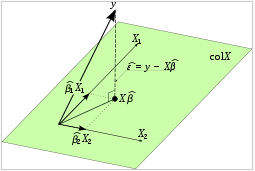
\includegraphics[height=2in]{OLS}}

\end{frame}

\begin{frame}
  \frametitle{Properties}
 $\Yhat = \muhat$ is an unbiased estimate of $\mub = \X\b$
\pause
    \begin{eqnarray*}
      \E [ \Yhat ]  & = & \E [\P_\X \Y ] \pause\\
& = & \P_\X \E[\Y] \pause\\
& = & \P_\X \mub \pause\\
& = & \mub \pause
    \end{eqnarray*}

$\E[\e] = \zero$ if $\mub \in C(\X)$ \pause
\begin{eqnarray*}
      \E [ \e ]  & = & \E [(\I - \P_\X) \Y ] \pause\\
& = & (\I - \P_\X) \E[\Y] \pause\\
& = & (\I - \P_\X) \mub \pause\\
& = & \zero \pause
    \end{eqnarray*}
Will not be $\zero$ if $\mub \notin C(\X)$

\end{frame}

\begin{frame}
  \frametitle{Estimate of $\sigma^2$}
MLE of $\sigma^2$:
  $$\shat = \frac{\e^T\e}{n} = \frac{\Y^T (\I - \P_\X) \Y}{n}$$
\pause
Is this an unbiased estimate of $\sigma^2$?
\pause

\vspace{1in}
Need expectations  of quadratic forms $\Y^T \A \Y$ for $\A$ an
 $n \times n$ matrix $\Y$ a random vector in $\bbR^n$
\end{frame}
\begin{frame}
  \frametitle{Quadratic Forms}
  Without loss of generality we can assume that $\A = \A^T$
\pause
  \begin{itemize}
  \item $\Y^T \A \Y$ is a scalar \pause
\item $\Y^T \A \Y  = (\Y ^T\A  \Y)^T = \Y^T \A^T \Y$ \pause
  \begin{eqnarray*}
 \frac{\Y^T \A \Y  + \Y^T \A^T \Y}{2} & = &
\Y^T \A \Y  \pause \\
    \Y^T\frac{(\A + \A^T)}{2}\Y  & = & \Y^T \A \Y \pause
  \end{eqnarray*}
\item may take $\A = \A^T$
  \end{itemize}
\end{frame}
\begin{frame}
  \frametitle{Expectations of Quadratic Forms}
  \begin{theorem}
   Let  $\Y$ be a random vector in $\bbR^n$ with $\E[\Y] = \mub$ and
   $\Cov(\Y) = \Sigmab$.  \pause Then $\E[\Y^T \A \Y] = \tr \A \Sigma + \mub^T
   \A \mub$.
  \end{theorem} \pause
Result useful for finding expected values of Mean Squares; no
normality required!
\end{frame}
\begin{frame}
  \frametitle{Proof}
Start with $(\Y - \mub)^T\A (\Y - \mub)$,  expand and take
expectations \pause
  \begin{eqnarray*}
\E [(\Y - \mub)^T\A (\Y - \mub)] & = & \E[\Y^T\A \Y + \mub^T\A \mub -
    \mu^T\A \Y - \Y^T \A \mu] \pause \\
 & = & \E[\Y^T\A \Y] + \mub^T\A \mub -
\mub^T\A \mub - \mub^T\A \mub \pause \\
 & = & \E[\Y^T\A \Y] - \mub^T\A \mub \pause 
  \end{eqnarray*}
Rearrange \pause
 \begin{eqnarray*}
 \E[\Y^T\A \Y ] & = &  \E[ (\Y - \mub)^T\A (\Y - \mub)] + \mub^T\A
 \mub \pause \\
 & = & \E[ \tr (\Y - \mub)^T\A (\Y - \mub)] + \mub^T\A \mub  \pause\\
 & = & \E[ \tr \A (\Y - \mub) (\Y - \mub)^T] + \mub^T\A
 \mub \pause \\
 & = &\tr  \E[ \A (\Y - \mub) (\Y - \mub)^T] + \mub^T\A \mub \pause \\
 & = &\tr \A \E([ (\Y - \mub) (\Y - \mub)^T] + \mub^T\A \mub \pause \\
 & = &\tr \A \Sigmab + \mub^T\A \mub  \pause
\end{eqnarray*}
\alert<12>{{\small{$\tr \A \equiv \sum_{i=1}^n a_{ii}$}}}
\end{frame}
\begin{frame}
  \frametitle{Expectation of $\shat$}
  
Use the theorem: \pause
\begin{eqnarray*}
\E[\Y^T (\I - \P_\X) \Y] & = &\tr (\I - \P_\X) \sigma^2 \I +
\mub^T(\I - \P_\X) \mub  \pause \\
 & = &  \sigma^2 \tr (\I - \P_\X) \pause \\
 & = & \sigma^2 r(\I - \P_\X) \pause\\
& = & \sigma^2 (n - r(\X)) \pause
\end{eqnarray*}


Therefore an unbiased estimate of $\sigma^2$ is $$\frac{\e^T\e}{n - r(\X)}$$
\pause

\begin{block}{Trace of a Projection Matrix}
If $\P$ is an orthogonal projection matrix, then its eigenvalues
$\lambda_i$ are
either zero or one with $\tr (\P) = \sum_i(\lambda_i) = r(\P)$
\end{block}

\end{frame}
\begin{frame}
  \frametitle{Spectral Theorem}
  \begin{theorem}
    If $\A$ ($n \times n$) is a symmetric real matrix  then there
    exists a  $\U$ ($n \times n$) such that $\U^T\U = \U \U^T = \I_n$
     and a diagonal matrix $\Lambdab$ with
    elements $\lambda_i$ such that $\A = \U \Lambdab \U^T$
  \end{theorem} \pause
  \begin{itemize}
  \item $\U$ is an orthogonal matrix; $\U^{-1} = \U^T$ \pause
  \item The columns of $\U$ from an Orthonormal Basis for $\bbR^n$ \pause
  \item rank of $\A$ equals the number of non-zero eigenvalues
    $\lambda_i$ \pause
  \item Columns of $\U$ associated with non-zero eigenvalues form an
    ONB for $C(\A)$ (eigenvectors of $\A$) \pause
\item $\A^p = \U \Lambdab^p \U^T$ (matrix powers) \pause
\item a square root of $\A > 0$ is $\U \Lambdab^{1/2}\U^T$ \pause
  \end{itemize}
\end{frame}
\begin{frame}
  \frametitle{Projections}
\begin{block}{Projection Matrix}
If $\P$ is an orthogonal projection matrix, then its eigenvalues
$\lambda_i$ are
either zero or one with $\tr (\P) = \sum_i(\lambda_i) = r(\P)$
\end{block} \pause
\begin{itemize}
\item   $\P = \U \Lambdab \U^T $  \pause
\item $\P = \P^2$  $\Rightarrow$ $\U \Lambdab \U^T\U \Lambdab \U^T =
  \U\Lambdab^2\U^T$  \pause
\item $\Lambdab = \Lambdab^2$ is true only for $\lambda_i = 1$ or
  $\lambda_i =0$  \pause
\item Since $r(\P)$ is the number of non-zero eigenvalues, $r(\P) =
  \sum \lambda_i = \tr(\P)$  \pause
\end{itemize}
$$\P = \left[\U_P \U_{P^\perp} \right] 
\left[
  \begin{array}{ll}
    \I_r & \zero \\
    \zero & \zero_{n-r}
  \end{array}
\right] \left[
  \begin{array}{l}
    \U_P^T \\
\U^T_{P^\perp}
  \end{array}
\right] = \U_P \U^T_P$$
$$\P = \sum_{i=1}^r \u_i \u_i^T$$  
sum of $r$ rank 1 projections.
\end{frame}


\begin{frame}[fragile]
  \frametitle{Prostate Example}
  \begin{small}
\begin{verbatim}
> library(lasso2)
> summary(lm(lcavol ~ ., data=Prostate))

Coefficients:
             Estimate Std. Error t value Pr(>|t|)    
(Intercept) -2.260101   1.259683  -1.794   0.0762 .  
lweight     -0.073166   0.174450  -0.419   0.6759    
age          0.022736   0.010964   2.074   0.0410 *  
lbph        -0.087449   0.058084  -1.506   0.1358    
svi         -0.153591   0.253932  -0.605   0.5468    
lcp          0.367300   0.081689   4.496 2.10e-05 ***
gleason      0.190759   0.154283   1.236   0.2196    
pgg45       -0.007158   0.004326  -1.654   0.1016    
lpsa         0.572797   0.085790   6.677 2.11e-09 ***
---

Residual standard error: 0.6998 on 88 degrees of freedom
Multiple R-squared:  0.6769,	Adjusted R-squared:  0.6475 
F-statistic: 23.04 on 8 and 88 DF,  p-value: < 2.2e-16
\end{verbatim}
    
  \end{small}

\end{frame}
\end{document}

\begin{frame}
  \frametitle{Independence or Zero Correlation}
\vspace{-10pt}
  \begin{eqnarray*}
    \Cov(\e, \muhat) & = & \Cov((\I - \P_\X)\Y, \P_\X \Y) \pause\\
 & = & (\I - \P_\X) \sigma^2 \I \P_\X^T \pause\\
 & = & \sigma^2 (\I - \P_\X) \P_\X \pause\\
& = & \sigma^2 (\P_\X - \P_\X\P_\X ) \pause\\
& = & \sigma^2 (\P_\X - \P_\X) \pause \\
& = & = \zero
  \end{eqnarray*}
Covariances of residuals \pause
  \begin{eqnarray*}
    \Cov(\e) & = & \Cov((\I - \P_\X)\Y) \pause \\
 & = & (\I - \P_\X) \sigma^2 \I (\I - \P_\X) ^T\pause \\
 & = & \sigma^2 (\I - \P_\X)(\I -  \P_\X) \pause\\
& = & \sigma^2 (\I_\X - \P_\X) \pause \\
  \end{eqnarray*}
$$ \e \sim \N(\zero_n, \sigma^2 (\I_n - \P_\X))$$
\end{frame}


\begin{frame}
  \frametitle{Generalize Inverses}

A generalize invers of $\A$: $\A^{-}$ satisfies   $\A \A^- \A = \A$


Special Case: Moore-Penrose Generalized Inverse  \pause


\begin{itemize}
\item Decompose symmetric $\A = \U \Lambdab \U^T$  \pause
\item $\A^-_{MP} = \U \Lambdab^- \U^T$  \pause
\item $\Lambdab^-$ is diagonal with $$ \lambda_i^- = \left\{
    \begin{array}{l}
   1/\lambda_i \text{ if } \lambda_i \neq 0 \\
   0 \quad \, \text{  if } \lambda_i = 0
    \end{array}
\right.$$  \pause
\item Symmetric  $\A^-_{MP} = (\A^-_{MP})^T $  \pause
\item Reflexive  $\A^-_{MP}\A \A^-_{MP} = \A^-_{MP} $  \pause
\end{itemize}

If $\P$ is an orthogonal projection matrix, the generalized inverse of
$\P$, $\P^- = \P$ 


\end{frame}
\begin{frame} \frametitle{Models \& MLEs}
  \begin{itemize}
  \item   $\Y \sim \N(\mub, \sigma^2 \I_n)$ with $\mub \in C(\X)
    \Leftrightarrow \mub = \X \b$  \pause
  \item   Claim: Maximum Likelihood Estimator (MLE) of $\mub$ is
    $\P_\X \Y$  \pause
\item $\P_\X$ is the orthogonal projection operator on the column
  space of $\X$; e.g. $\X$ full rank $\P_\X = \X (\X^T\X)^{-1} \X^T$
  \pause
\item If $\X^T\X$ is not invertible use a generalized inverse
\end{itemize}
\begin{lemma}[B.43]
  If $\, \G$ and $\H$ are generalized inverses of $(\X^T\X)$ then
  \begin{enumerate}
  \item $\X \G \X^T \X = \X \H \X^T \X = \X$
  \item $\X \G \X^T = \X \H \X^T$
  \end{enumerate}
\end{lemma} \pause
$\P_\X = \X (\X^T\X)^{-} \X^T$ is the orthogonal projection operator
onto $C(\X)$   (does not depend on choice of generalized inverse!)
[See proof in Theorem B.44]
\end{frame}

\begin{frame}
  \frametitle{Identifiability}
$\Y \sim \N(\mub, \sigma^2 \I)$  \pause
  \begin{itemize}
  \item Distribution of $\Y$ determined by $\mub$ and $\sigma^2$  \pause
\item $\mub = \X\b = \mu(\b)$  \pause
\end{itemize}
  \begin{block}{Identifiability}
$\b$ and $\sigma^2$ are identifiable if distribution of $\Y$, $f_\Y(\y;
\b_1, \sigma^2_1) = f_\Y(\y;
\b_2, \sigma^2_2)$ implies that $(\b_1, \sigma^2_1)^T =  (\b_2, \sigma^2_2)^T$
  \end{block}  \pause
For linear models, equivalent definition is that $\b$ is identifiable
if for any $\b_1$ and $\b_2$ $\mu(\b_1) = \mu(\b_2)$ implies that
$\b_1 = \b_2$.  If $ r(\X) = p$ then $\b$ is identifiable
 \pause
\vspace{12pt}
If $\X$ is not full rank, there exists $\b_1 \neq \b_2$, but $\X\b_1 = \X\b_2$
\end{frame}

\begin{frame}
  \frametitle{MLE of $\b$}
  \begin{eqnarray*}
    \P_\X \Y & = & \X \bhat  \\
\X(\X^T\X)^- \X^T\Y & =
& \X \bhat 
  \end{eqnarray*}  \pause
  \begin{itemize}
\item If $\X^T\X$ is invertible, then
$$\bhat = (\X^T\X)^{-1} \X^T\Y$$ and is unique  \pause

\item But if $\X^T\X$ is  not invertible, $$\bhat = (\X^T\X)^{-} \X^T\Y$$ is
one solution which depends on choice of generalized inverse
 \pause
  \end{itemize}

What can we estimate uniquely?
\end{frame}
\begin{frame}
  \frametitle{Non-Identifiable }
  Recall the Oneway ANOVA model \pause
$$\mu_{ij} = \mu + \tau_j$$ \pause
\begin{itemize}
\item Let $\b_{1} = (\mu, \tau_1, \ldots, \tau_J)^T$ \pause
\item Let $\b_{2} = (\mu - 42, \tau_1 + 42, \ldots, \tau_J + 42)^T$ \pause
\item Then $\mub_{1} = \mub_{2}$ even though different values of the
  parameters  $\b_1 \neq \b_2$ \pause
\item $\b$ is not identifiable \pause
\item $\mub$ is identifiable, yet $\mub = \X \b$  (a linear
  combination of $\b$) \pause
\item Next class: what parameters  or combinations of parameters can we estimate?
\end{itemize}

\end{frame}